\documentclass[12pt,a4paper]{article}

% ── Packages ──────────────────────────────────────────────────────────────────
\usepackage[margin=1in]{geometry}
\usepackage{times}
\usepackage{amsmath,amssymb}
\usepackage{graphicx}
\usepackage{booktabs}
\usepackage{array}
\usepackage{caption}
\usepackage{subcaption}
\usepackage{float}
\usepackage[hidelinks]{hyperref}
\usepackage{parskip}
\usepackage{setspace}
\usepackage{fancyhdr}
\usepackage{titlesec}
\usepackage[table]{xcolor}

% ── Page style ────────────────────────────────────────────────────────────────
\pagestyle{fancy}
\fancyhf{}
\rhead{CPSC 3180/5180 Final Project}
\lhead{Chang Zhang}
\cfoot{\thepage}

\setstretch{1.15}

\titleformat{\section}{\large\bfseries}{\thesection}{1em}{}
\titleformat{\subsection}{\normalsize\bfseries}{\thesubsection}{1em}{}

% ── Document ──────────────────────────────────────────────────────────────────
\begin{document}

% ── Title page ────────────────────────────────────────────────────────────────
\begin{titlepage}
  \centering
  \vspace*{2cm}
  {\LARGE\bfseries YouTube Viral Video Prediction\\[0.4em]
  Using Pre-Publication Information\par}
  \vspace{1.5cm}
  {\large Yale University\\
  CPSC 3180/5180: Introduction to Machine Learning\\
  Spring 2026\par}
  \vspace{1cm}
  {\large Instructor: Alex Wong\par}
  \vspace{1cm}
  {\large\bfseries Chang Zhang\par}
  \vfill
\end{titlepage}

% ── Abstract ──────────────────────────────────────────────────────────────────
\begin{center}\large\bfseries Abstract\end{center}
This project investigates whether a YouTube video's virality can be predicted
using only information available before publication: the video title, publish
timestamp, and content category.  We define a video as viral if its view count
reaches the 80th percentile among videos in the dataset, yielding a binary
classification task with roughly 20\% positive examples.  Two models are
compared: a Logistic Regression baseline trained on five structured features,
and an RBF Kernel SVM trained on the same structured features augmented with
TF-IDF title representations.  The SVM achieves an AUC of 0.655 and an F1
score of 0.378, compared to 0.558 and 0.296 for the baseline, suggesting that
title text provides meaningful additional predictive signal.  A cross-category
generalization experiment further reveals that viral patterns are strongly
category-specific, with in-domain F1 averaging 0.657 and cross-domain F1
averaging 0.198, an insight that points toward category-aware modeling as a
natural direction for future work.

\noindent\textbf{Keywords:} viral prediction, TF-IDF, logistic regression, kernel SVM, PCA

\vspace{1em}
\tableofcontents
\newpage

% ── 1. Introduction ───────────────────────────────────────────────────────────
\section{Introduction}

Predicting whether a YouTube video will go viral is a problem of practical
interest to content creators, platform operators, and marketers.  Most
approaches to this problem rely on post-publication engagement signals such as
view counts, likes, and comment volume --- metrics that are only observable
after a video has already been released and seen by an audience.  This project
poses a stricter and more realistic question: \textit{can we predict virality
using only information that exists at the moment of upload?}

The features considered are limited to the video title, publish timestamp, and
content category, all of which are determined before a video goes live.
Engagement metrics (views, likes, dislikes, comment count) are explicitly
excluded as model inputs; view counts are used solely for constructing the
binary viral label.

Beyond the core prediction task, the project investigates a second question:
\textit{do viral patterns generalize across content categories?}  A model
trained on Gaming videos may have learned patterns specific to that genre.
Testing whether those patterns transfer to Music or Entertainment reveals
whether virality is a universal phenomenon or a category-specific one --- a
question with direct implications for how such models should be designed and
deployed in practice.

Two main experiments are conducted.  Experiment~1 trains a Logistic Regression
classifier on structured features only to establish a baseline.  Experiment~2
augments these features with a TF-IDF representation of the video title and
trains an RBF Kernel SVM, testing whether the specific words in a title carry
additional predictive power.  Two further experiments visualize the learned
feature space via PCA and measure cross-category generalization through a
held-out F1 matrix.

% ── 2. Data ───────────────────────────────────────────────────────────────────
\section{Data}

\subsection{Dataset}

The dataset used is the \textbf{Kaggle Trending YouTube Video Statistics} (US
subset), consisting of a CSV file of video records and a JSON category mapping
file.  It contains metadata for videos that appeared on YouTube's US trending
page, including the video title, publish timestamp, category identifier, view
count, like count, dislike count, and comment count.  The raw dataset contains
40,949 rows.  Because the same video can appear on multiple trending days, we
deduplicate by video identifier and retain only the first appearance of each
video, reducing the dataset to 6,351 unique videos.  After removing rows with
missing titles or unparseable publish timestamps, all 6,351 samples are
retained.

\subsection{Label Definition}

A binary viral label is constructed from view counts:
\[
  \text{viral} =
  \begin{cases}
    1 & \text{if } \text{views} \geq Q_{0.80}(\text{views}) \\
    0 & \text{otherwise}
  \end{cases}
\]
where $Q_{0.80}$ denotes the 80th percentile of the view count distribution
(933,053 views).  This yields approximately 20\% positive (viral) examples,
providing a more balanced class distribution for model training.

\subsection{Category Distribution}

To understand the data, we computed the viral rate for each content category.
Categories vary substantially in their fraction of viral videos, as shown in
Figure~\ref{fig:viral_by_category}, suggesting that category identity carries
meaningful signal for prediction.

\begin{figure}[H]
  \centering
  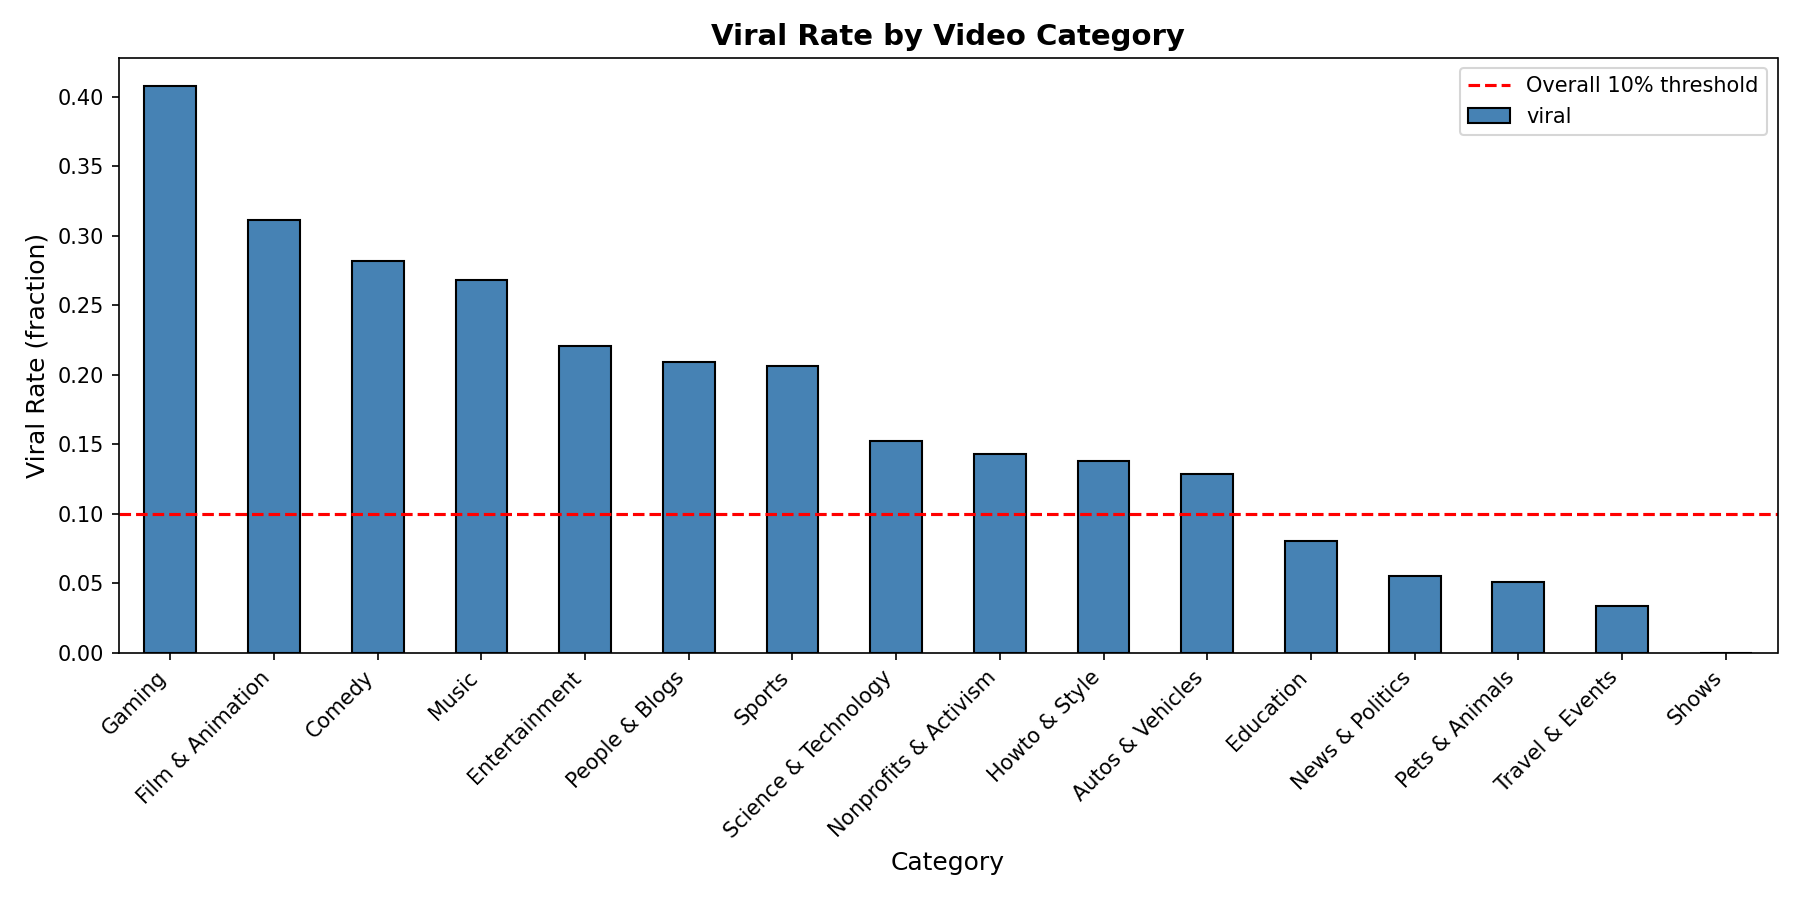
\includegraphics[width=0.85\textwidth]{phase1_viral_rate_by_category.png}
  \caption{Viral rate broken down by YouTube content category.
           The dashed red line marks the overall 10\% baseline.}
  \label{fig:viral_by_category}
\end{figure}

% ── 3. Methodology ────────────────────────────────────────────────────────────
\section{Methodology}

\subsection{Feature Engineering}

Two feature sets are constructed from the allowed input variables.

\textbf{Structured features} (5 dimensions):
\begin{itemize}
  \item publish hour --- hour of day (0--23) extracted from the publish timestamp
  \item publish weekday --- day of week (0 = Monday, 6 = Sunday)
  \item title length --- number of characters in the title
  \item title word count --- number of whitespace-delimited tokens in the title
  \item category id --- integer category identifier
\end{itemize}

\textbf{Text features:}  A TF-IDF representation of the video title is
computed with a vocabulary limited to the top 500 terms (English stop words
removed), yielding a 500-dimensional sparse vector per video.

The full feature matrix concatenates the scaled structured features and the
TF-IDF vector, producing a 505-dimensional representation.  To prevent data
leakage, the standard scaler for structured features, the TF-IDF vectorizer,
and the PCA transform used in Experiment~2 are all fitted exclusively on the
training split and then applied to the test split.

\subsection{Train/Test Split}

The dataset is divided into a 70\% training set and a 30\% test set using
stratified sampling (preserving the viral/non-viral ratio in both splits) with
a fixed random seed for reproducibility.

\subsection{Experiment 1 --- Logistic Regression Baseline}

Logistic Regression with $\ell_2$ regularization is trained on the structured
features only.  The model minimizes the regularized cross-entropy loss:
\[
  \min_{w,b} \;\sum_{i=1}^{n}
    \log\!\left(1 + e^{-y_i(w^\top x_i + b)}\right)
  + \frac{1}{2C}\|w\|^2
\]
where $C > 0$ controls regularization strength (larger $C$ = less
regularization).  Class imbalance is handled by reweighting each training
example inversely proportional to its class frequency.  The optimal $C$ is
selected via 5-fold stratified cross-validation over the grid
$C \in \{0.001,\ 0.01,\ 0.1,\ 1,\ 10\}$, with F1 score as the selection criterion.

\subsection{Experiment 2 --- RBF Kernel SVM}

A Support Vector Machine with the Radial Basis Function (RBF) kernel is trained
on the full feature set.  Because the SVM's computational cost scales poorly
with the number of features, PCA first reduces the 505-dimensional feature
matrix to 100 principal components.  The RBF kernel implicitly maps inputs into
a high-dimensional feature space:
\[
  K(x_i, x_j) = \exp\!\left(-\gamma\,\|x_i - x_j\|^2\right)
\]
The SVM then finds the maximum-margin separating hyperplane in this space.
Hyperparameters $C \in \{0.1,\,1,\,10\}$ and
$\gamma \in \{\text{scale},\,0.01,\,0.1\}$ are jointly tuned via 5-fold
cross-validation optimizing F1.  Class imbalance is handled identically to
Experiment~1.

\subsection{Experiment 3 --- PCA Visualization}

To examine the geometry of the feature space, PCA is applied to project the
full training feature matrix to 2 dimensions.  Viral and non-viral samples are
plotted separately to assess visual separability, both for the full training set
and individually for four categories: Gaming, Music, Entertainment, and Science
\& Technology.

\subsection{Experiment 4 --- Cross-Category Generalization}

To assess whether viral patterns transfer across content genres, the four most
frequent categories are selected.  For each ordered pair (train category, test
category), a separate SVM is trained on all samples from the training category
and evaluated on all samples from the test category using the best
hyperparameters from Experiment~2.  This produces a $4\times4$ F1 matrix whose
diagonal entries represent in-domain performance and whose off-diagonal entries
represent cross-domain generalization.

% ── 4. Implementation Details ─────────────────────────────────────────────────
\section{Implementation Details}

All experiments are implemented in Python~3 using scikit-learn.
Table~\ref{tab:impl} summarizes the key hyperparameter settings.

\begin{table}[H]
  \centering
  \caption{Implementation settings used across all experiments.}
  \label{tab:impl}
  \begin{tabular}{ll}
    \toprule
    \textbf{Setting} & \textbf{Value} \\
    \midrule
    Unique videos (after deduplication) & 6,351 \\
    Train / test split ratio  & 70 / 30, stratified \\
    Viral label threshold     & 80th percentile (933,053 views), 20\% positive \\
    Random state              & 42 (all steps) \\
    TF-IDF vocabulary size    & 500 \\
    TF-IDF stop words         & English \\
    PCA components (Exp.\ 2)  & 100 \\
    LR solver                 & L-BFGS, max iterations = 1000 \\
    LR best $C$               & 0.001 \\
    LR $C$ grid               & $C \in \{0.001,\,0.01,\,0.1,\,1,\,10\}$ \\
    SVM kernel                & RBF \\
    SVM best params           & $C=10$, $\gamma=0.1$ \\
    SVM $C$ grid              & $\{0.1,\,1,\,10\}$ \\
    SVM $\gamma$ grid         & $\{\text{scale},\,0.01,\,0.1\}$ \\
    Cross-validation folds    & 5-fold stratified \\
    CV scoring metric         & F1 \\
    Class imbalance handling  & Inverse-frequency sample weighting \\
    Leakage prevention        & Scaler / TF-IDF / PCA fit on training set only \\
    \bottomrule
  \end{tabular}
\end{table}

% ── 5. Results ────────────────────────────────────────────────────────────────
\section{Results}

\subsection{Experiment 1 --- Logistic Regression Baseline}

We trained a Logistic Regression model using only the five structured features
and evaluated it on the held-out test set.  The best regularization parameter
found by cross-validation was $C = 0.001$.  Inspecting the learned coefficient
vector revealed that category id and publish weekday carry the largest absolute
weights, suggesting that content category and day of week encode the most
useful signal among the structured features.

The model achieves a recall of 0.451, identifying roughly 45\% of viral videos,
but precision is low at 0.220, indicating a high false-positive rate.  The AUC
of 0.558 is only modestly above random chance (0.5), establishing the limited
ceiling of what structured features alone can offer and motivating the addition
of text features in Experiment~2.  Figure~\ref{fig:lr} shows the ROC curve and
confusion matrix.

\begin{figure}[H]
  \centering
  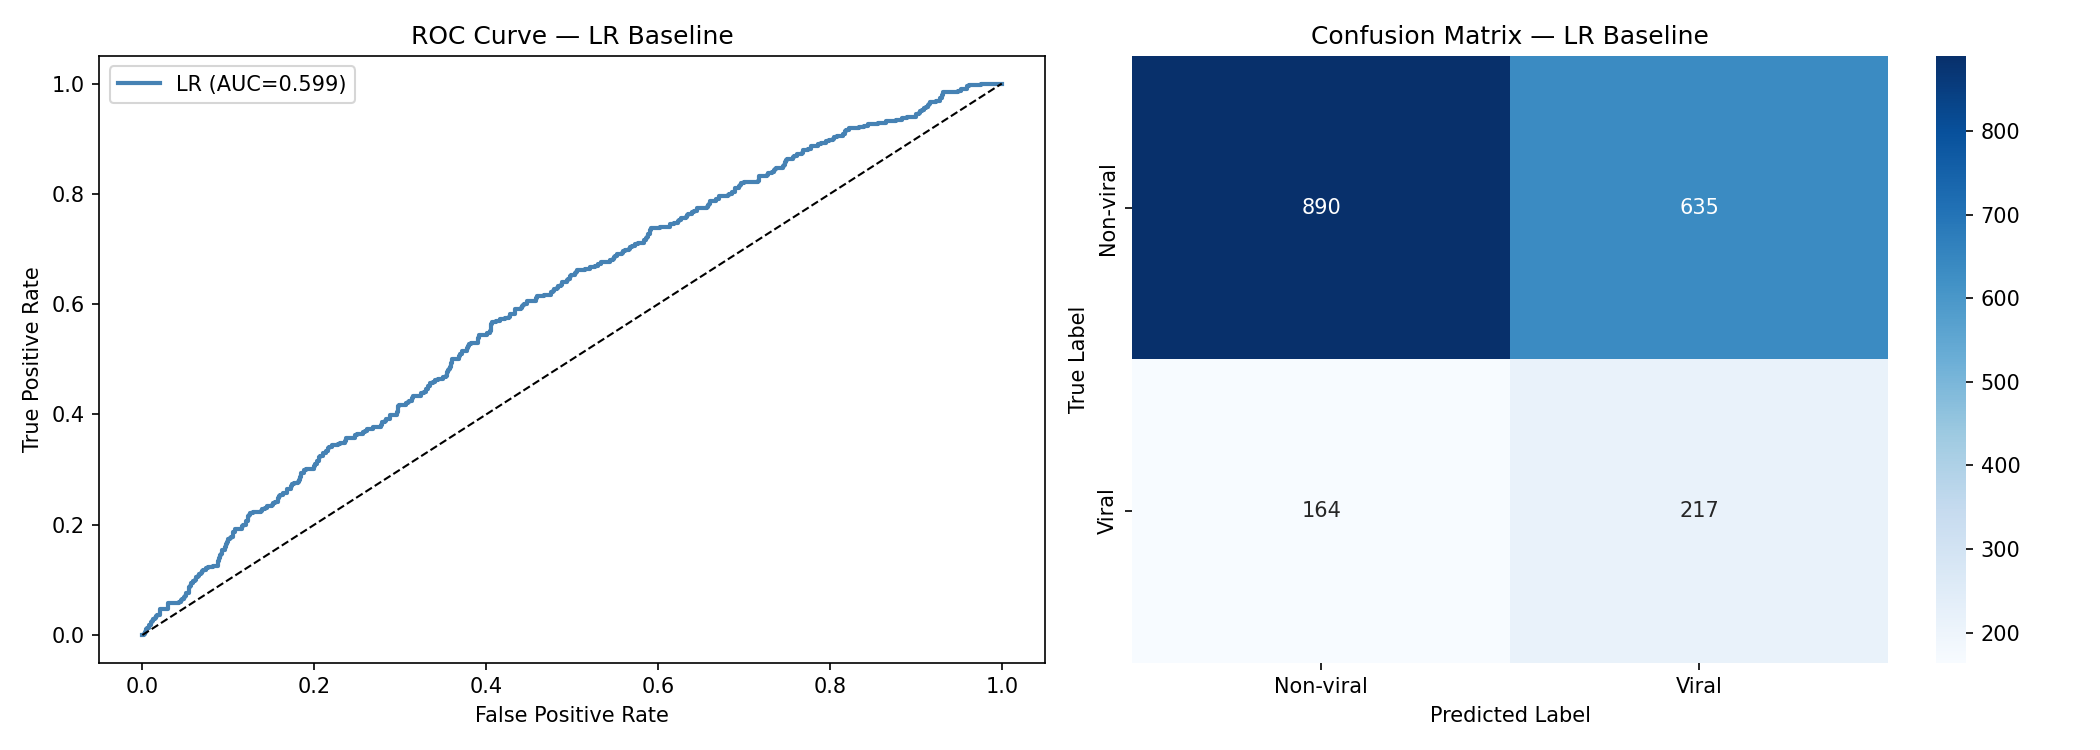
\includegraphics[width=0.88\textwidth]{phase3_lr_baseline.png}
  \caption{Logistic Regression baseline results: ROC curve (left) and confusion
           matrix (right) on the held-out test set.}
  \label{fig:lr}
\end{figure}

\subsection{Experiment 2 --- Kernel SVM}

We augmented the structured features with TF-IDF title representations, applied
PCA to reduce dimensionality to 100 components (retaining 91.69\% of variance),
and trained an RBF Kernel SVM.  Cross-validation selected $C = 10$ and
$\gamma = 0.1$ as the best hyperparameters.

The results, summarized in Table~\ref{tab:results}, show clear improvement
across every metric.  F1 increases by 28.0\% relative to the baseline, and AUC
reaches 0.655.  Recall of 0.504 means the model correctly identifies roughly
half of all truly viral videos, while precision improves from 0.220 to 0.303.
Although the absolute performance is moderate, the consistent gains across all
metrics suggest that title text provides genuine predictive signal beyond what
structured features alone can capture.  Part of the improvement may also reflect
the greater flexibility of the RBF kernel compared to a linear classifier,
though the feature addition is the primary driver.

\begin{table}[H]
  \centering
  \caption{Test set performance of the two models.}
  \label{tab:results}
  \renewcommand{\arraystretch}{1.2}
  \begin{tabular}{lccccc}
    \toprule
    \textbf{Model} & \textbf{Accuracy} & \textbf{Precision} &
    \textbf{Recall} & \textbf{F1} & \textbf{AUC} \\
    \midrule
    LR Baseline (structured only)        & 0.570 & 0.220 & 0.451 & 0.296 & 0.558 \\
    Kernel SVM (structured + TF-IDF)     & 0.669 & 0.303 & 0.504 & 0.378 & 0.655 \\
    \midrule
    \rowcolor{gray!15}
    Absolute improvement ($\Delta$)      & +0.099 & +0.083 & +0.053 & +0.082 & +0.097 \\
    \rowcolor{gray!15}
    Relative improvement (\%)            & +17.4\% & +37.7\% & +11.8\% & +27.7\% & +17.4\% \\
    \bottomrule
  \end{tabular}
\end{table}

Figure~\ref{fig:svm} provides the ROC comparison, SVM confusion matrix, and a
side-by-side metric bar chart for both models.

\begin{figure}[H]
  \centering
  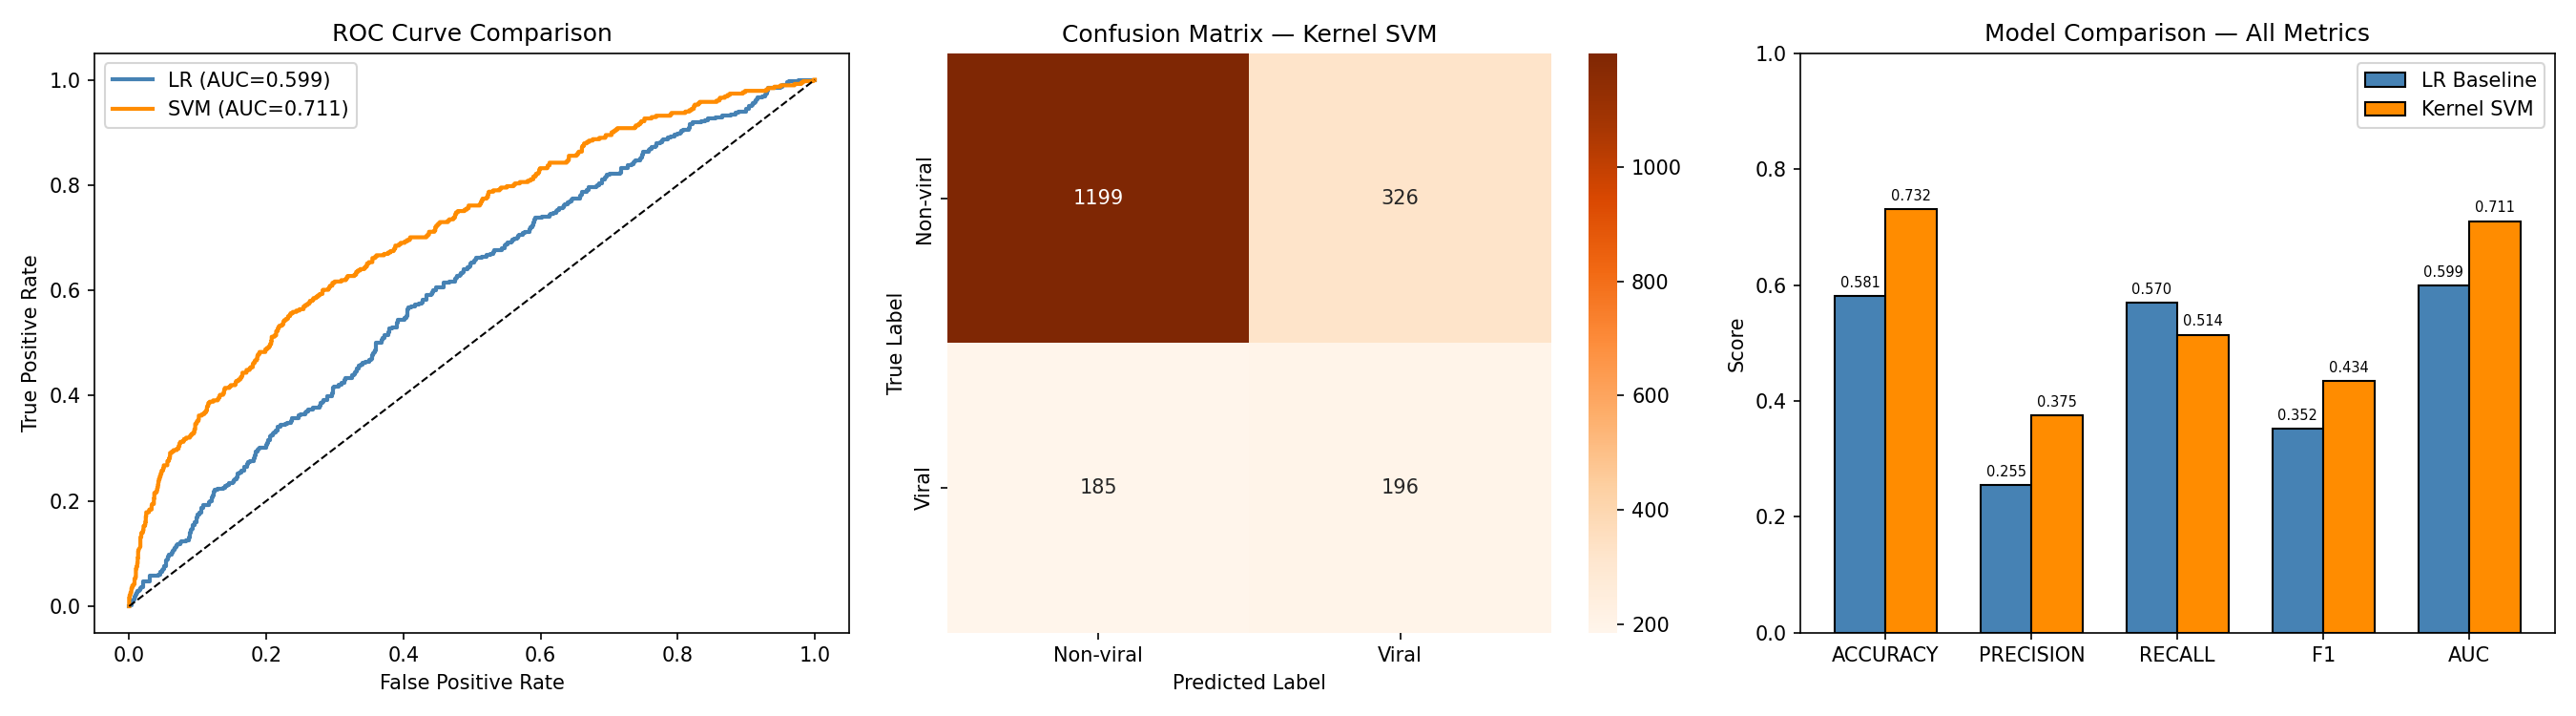
\includegraphics[width=\textwidth]{phase4_svm_comparison.png}
  \caption{Experiment 2 results: ROC curve comparison (left), SVM confusion
           matrix (center), and per-metric bar chart comparing LR and SVM
           (right).}
  \label{fig:svm}
\end{figure}

\subsection{Experiment 3 --- PCA Visualization}

To gain intuition about the feature space, we projected the 505-dimensional
training features down to 2 principal components and plotted viral versus
non-viral samples.  While the two classes overlap to some degree --- expected
given the inherent difficulty of the task --- viral videos occupy a noticeably
distinct region along the first principal component, confirming that the learned
features carry genuine discriminative signal.

The per-category breakdown, shown in Figure~\ref{fig:pca_cat}, reveals
meaningful variation across genres.  Table~\ref{tab:pca} reports the Euclidean
distance between the viral and non-viral cluster centroids in 2D PCA space for
each category.  Gaming and Entertainment exhibit the clearest separation, while
Music videos cluster tightly regardless of virality, consistent with the
difficulty of predicting viral Music content from title features alone.

\begin{figure}[H]
  \centering
  \includegraphics[width=0.75\textwidth]{phase5_pca2d_overall.png}
  \caption{PCA 2D projection of the full training set.  Orange points are viral
           videos; blue points are a random subsample of 2,000 non-viral videos.}
  \label{fig:pca_overall}
\end{figure}

\begin{figure}[H]
  \centering
  \includegraphics[width=\textwidth]{phase5_pca2d_by_category.png}
  \caption{Per-category PCA 2D projections for Gaming, Music, Entertainment,
           and Science \& Technology.}
  \label{fig:pca_cat}
\end{figure}

\begin{table}[H]
  \centering
  \caption{Centroid distance between viral and non-viral clusters in 2D PCA
           space, by category.}
  \label{tab:pca}
  \begin{tabular}{lcc}
    \toprule
    \textbf{Category} & \textbf{Centroid Distance} & \textbf{Separation} \\
    \midrule
    Gaming                & 0.444 & Clear \\
    Entertainment         & 0.208 & Moderate \\
    Science \& Technology & 0.365 & Moderate \\
    Music                 & 0.035 & Weak \\
    \bottomrule
  \end{tabular}
\end{table}

\subsection{Experiment 4 --- Cross-Category Generalization}

To understand how well viral patterns transfer across genres, we trained
separate SVM models on each of the four most frequent categories ---
Entertainment, Music, Howto \& Style, and Comedy --- and tested each model on
every category, yielding the $4 \times 4$ F1 matrix in
Figure~\ref{fig:heatmap}.  The diagonal entries (in-domain) average 0.657,
confirming that category-specific models learn meaningful patterns within their
own genre.  The off-diagonal entries (cross-domain) average 0.198, a drop of
0.459.

This gap reveals an important structural property of the data: viral patterns
are largely category-specific.  The language and framing that makes an
Entertainment title go viral differs substantially from what works in Music or
Howto \& Style.  Music is the most category-specific genre --- models trained
on Music generalize least to other categories, consistent with the weak PCA
separation observed in Experiment~3.

\begin{figure}[H]
  \centering
  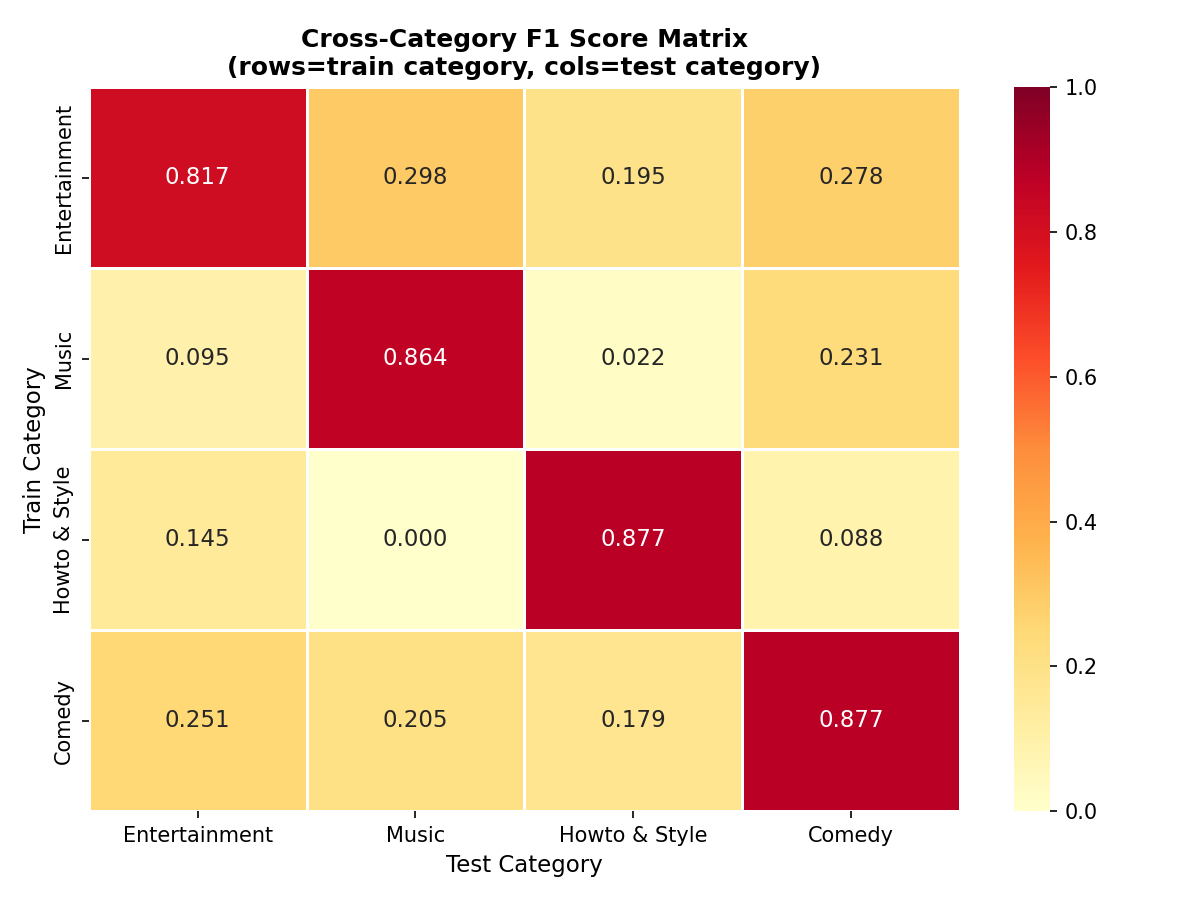
\includegraphics[width=0.65\textwidth]{phase6_cross_category_heatmap.png}
  \caption{Cross-category F1 matrix.  Rows indicate the training category;
           columns indicate the test category.  Diagonal entries are in-domain
           results; off-diagonal entries are cross-domain results.}
  \label{fig:heatmap}
\end{figure}

% ── 6. Discussion ─────────────────────────────────────────────────────────────
\section{Discussion}

\textbf{Viral video prediction from pre-publication features is feasible.}
The Kernel SVM achieves an AUC of 0.655 and an F1 of 0.378 using only title
text, publish time, and content category --- no engagement data whatsoever.
While the absolute numbers reflect the genuine difficulty of the task, both
metrics improve meaningfully over the structured-only baseline (AUC 0.558,
F1 0.296), confirming that pre-publication signals carry real predictive value.

\textbf{Title text provides meaningful additional signal.}  The 28\% relative
improvement in F1 from the structured-only baseline to the text-augmented SVM
suggests that the specific words a creator chooses matter beyond timing and
category.  This is an actionable finding: title optimization is a concrete lever
available to creators before a video is ever published.

\textbf{Viral patterns are category-specific, which is itself a useful
finding.}  The cross-category experiment was designed to ask whether a single
global model would be sufficient.  The answer is no --- in-domain F1 averages
0.657 while cross-domain F1 averages only 0.198.  But this is not a failure of
the model; it is a discovery about the nature of virality on YouTube: different
genres have different linguistic cultures, and what goes viral in one does not
necessarily go viral in another.  Knowing this guides how future systems should
be built --- with separate, category-aware models rather than a single
one-size-fits-all classifier.

\textbf{Practical implications.}  These findings translate into concrete
guidance for content creators.  First, since title text is the strongest
predictive signal, investing effort in title wording --- choosing specific,
evocative language rather than generic descriptions --- is likely to have the
greatest impact on a video's reach.  Second, because publish hour and weekday
are among the most informative structured features, timing uploads strategically
(e.g., aligning with peak audience activity periods) provides an additional
marginal advantage.  Third, the category-specific nature of viral patterns means
that creators should study what works within their own genre rather than
emulating strategies from unrelated categories --- a title style that performs
well in Science \& Technology may be counterproductive in Music.  Finally, the
trained model itself can serve as a practical pre-upload screening tool: given a
candidate title, publish time, and category, it can estimate the probability of
going viral before a video is ever released, enabling iterative title refinement
at zero cost.

\textbf{Future directions.}  Building on these results, natural extensions
include training dedicated per-category models, exploring richer text
representations such as pretrained sentence embeddings, and incorporating
additional pre-publication signals such as channel subscriber count or thumbnail
features.

% ── 7. Conclusion ─────────────────────────────────────────────────────────────
\section{Conclusion}

This project demonstrates that predicting YouTube video virality from
pre-publication information alone is feasible.  By combining structured metadata
with TF-IDF title features and training an RBF Kernel SVM, we achieve an AUC
of 0.655 and an F1 score of 0.378 on a held-out test set --- a 28\% improvement
in F1 over the structured-only Logistic Regression baseline.  The title text of
a video provides the strongest marginal signal among the available pre-publication
features.

The cross-category generalization experiment adds a deeper insight: viral
patterns are not universal but genre-dependent, with in-domain F1 averaging
0.657 and cross-domain F1 averaging 0.198.  Rather than undermining the
project's success, this finding clarifies the right modeling strategy going
forward --- category-aware models that respect the distinct linguistic norms of
each genre.  Together, these results demonstrate that machine learning can
extract meaningful structure from simple pre-publication metadata, with
practical implications for content strategy and platform design.


\end{document}
